\chapter{Introduction}\label{chap_intro}

For all our advances in modern medicine, we still don't understand what happens in the human brain and how it breaks down in a wide variety of mental illnesses. A 2010 study found that in England alone, mental illness directly affected one in six of us, with it costing the nation over £105bn per year\footnote{\url{http://www.centreformentalhealth.org.uk/economic-and-social-costs-2009}}. 20\% of that is the cost to the NHS and social care and 50\% being the financial burden it brings on families and the patients themselves. These figures are set to rise with a growing and ageing population, and so we need to develop a better understanding of how the brain works, and what changes during mental illness for better targeted treatment. Currently, our primary tool for diagnoses of mental health conditions comes from the surveying of symptoms which have been catalogued in texts such as the Diagnostic and Statistical Manual \citep{APA2013}. Whilst this has led to increased rates of diagnosis in patients and can aid in directed treatment, this is not always an entirely rigorous scientific process. For example, changing the criteria for diagnosis can have a profound effect on the number of reported cases of a condition; which is estimated to explain 30 \% of recent diagnoses of Autistic Spectrum Disorders in Danish children \citep{Hansen2015}. In addition, being able to stratify via clinical interviews does not necessarily explain the biological causes of conditions, for this we need to probe the brain to discover the potential origins of mental health disorders. Our understanding of the brain can be broadly categorised into three domains, the structural, the biochemical and the functional. All three are intrinsically linked, and so we need to better our understanding in each domain to truly understand how the brain operates and why it is perturbed. Non-invasive techniques in functional neuroimaging proves a popular avenue of research as they can be potentially used to identify \textit{where} in the brain disorders are specifically affecting, without the potential risks associated with invasive procedures. Knowing where a condition affects would allows future research to focus on \textit{why}, which could lead to a better informed diagnoses and improved targeted treatment. 

Since the days of Hippocrates we have been aware that the brain was the major controlling centre of the body, and for centuries humankind has been striving to understand the internal workings of the brain. Our work in characterising human brain function in a truly scientific manner dates back to the early 19th century; the first theory which resembles our 'modern' view of the brain originates from field of phrenology. A theory of the brain was hypothesised by Franz Joseph Gall in the early 19\textsuperscript{th} century, who postulated that the brain was made up of a complex series of 'mental organs', each with their own unique functions (different aspects of human personality) and were discretely localised within the cortex. Whilst we have come to realise phrenology is pseudoscientific, the notion of \textit{functional segregation} still exists today. The first experimental proof of this came in 1861, when a French neuroscientist by the name of Paul Broca, made the connection between two patients who suffered with aphasia (a disorder which affects speech and language), and lesions located in on their left frontal lobes \citep{Broca1861}. Over the years much work was done to investigate the locations of other brain functions using invasive recordings in both humans and animals, but most results showed a great deal of inconsistency with each other. However, successful efforts were made in mapping cortical function with invasive testing, most famously by Wilder Penfield who managed to map the motor and somatosensory cortices on patients who were in surgery \citep{Penfield1954}.

However the major breakthroughs in functional mapping, came along via new methods to non-invasively investigate brain function. The first of these came in 1924, when Hans Berger showed that it was possible to measure spontaneous fluctuations in electrical potentials on the scalp. This was first electrocencephalograph (EEG; \citealp{Berger1929}) and the first truly non-invasive measurement of brain function. The late 20\textsuperscript{th} Century saw the invention of x-ray computed tomography (CT), positron emission tomography (PET; \citealp{Fox1984}) and magnetic resonance imaging (MRI; \citealp{Lauterber1973,Mansfield1973}). In the 1980s, the combination of CT and PET allowed, for the first time, simultaneous anatomical and functional data collection, allowing us to map brain activity associated with heightened blood flow to regions of brain activity for the first time. However PET requires the insertion of a radioactive isotope into a patient as a marker. This, along with the fact it has poor spatiotemporal resolution, meant uses for exploratory investigations were limited. However MRI carries no such risks for subjects and has a vastly improved spatial and temporal resolution, the latter from the invention of echo planar imaging, which images the entire brain volume in a few hundred milliseconds \citep{Mansfield1977}. This combined with the discovery by Ogawa and colleagues in 1990 that blood could be used as an endogenous contrast to measure brain function, led to the birth of functional magnetic resonance imaging (fMRI; \citealp{Ogawa1990}). With the ubiquity of MRI systems due to the other clinical applications it possessed, the field of functional neuroimaging exploded in the 1990s. 

\section{Introducing functional connectivity}
%\citep{Friston1998,Schnitzler2005,Palaniyappan2012,Kessler2014}
Whilst headways were being made into the spatial origins of functional processes, a new facet to functional neuroimaging started to be investigated in the late 20\textsuperscript{th} Century, known as \textit{functional connectivity}. This new approach was defined as the \textit{'temporal correlation between remote neurophysiological events'} \citep{Friston1994} and stated that should the temporal profile of neural activity measured independently at two distal regions share a statistical interdependency, they are said to be working in concert. A simple example of a functional connection is this; if you were trying to catch a ball, the visual cortex which is processing the information about the ball's position and velocity needs to share this information with the motor cortices to dictate how you need to move to take a catch. The communication between these two otherwise separate regions is a functional connection. An understanding of these connections is of great importance, as it is hypothesised that communication within the brain facilitates healthy congition, and in clinical populations these connections may be perturbed. For example, an important
hypothesis underlying symptoms of schizophrenia is one of dysconnectivity between regions \citep{Friston1998}, and recent work has shown that connections between the bilateral insula and cingulate cortices, regions associated with salience, are abnormal in schizophrenia patients compared to healthy controls \citep{Palaniyappan2012}. This is one of many observations implicating abnormal functional connections in diseases ranging from developmental disorders \citep{Tomasi2012,Maccotta2013,Haneef2014,Kessler2014} to neurodegeneration \citep{Grady2001,Allen2007,Wang2007,Hawellek2011,Hacker2012,Leavitt2014}.

As functional connections are so wide ranging, non-invasive techniques which allow whole brain coverage prove to be the most useful modalities. The mapping of functional connections within the human brain was initially performed using PET \citep{Friston1991,Friston1993} which could show regions of covariant activation. However the short half-life of the radiolabel \textsuperscript{15}O (122 s) along with its ionising properties meant acquisition of experimental data in healthy individuals was limited. It was the landmark study by \cite{Biswal1995}, which demonstrated that fMRI, with its better spatial resolution and non-invasive nature, would allow research into functional connectivity to become the field it is today. What Biswal and his colleagues found was that by placing a seed in the motor cortex, even in the absence of a task, correlations existed between blood oxygen level dependent (BOLD) timecourses between the left and right motor cortices. By placing seeds in other regions of interest (ROIs) in the brain, further studies revealed a small number of robust, large scale networks connected brain regions in what are known as \textit{functional networks} or \textit{resting state networks} (RSNs; \citealp{Corbetta1998,Raichle2001,Beckmann2005,Fox2005,Fox2007,Smith2009}). These networks, each with their own characteristic spatial signature, are thought to govern core mental processes with some supporting sensory integration and others associated with cognition or attention. Most networks are observed even in subjects at rest, hence the RSN terminology. Example network topographies derived from a study by \cite{Smith2009} can be found in Figure \ref{fig_intro_1}.


\begin{figure}
	\begin{center}
		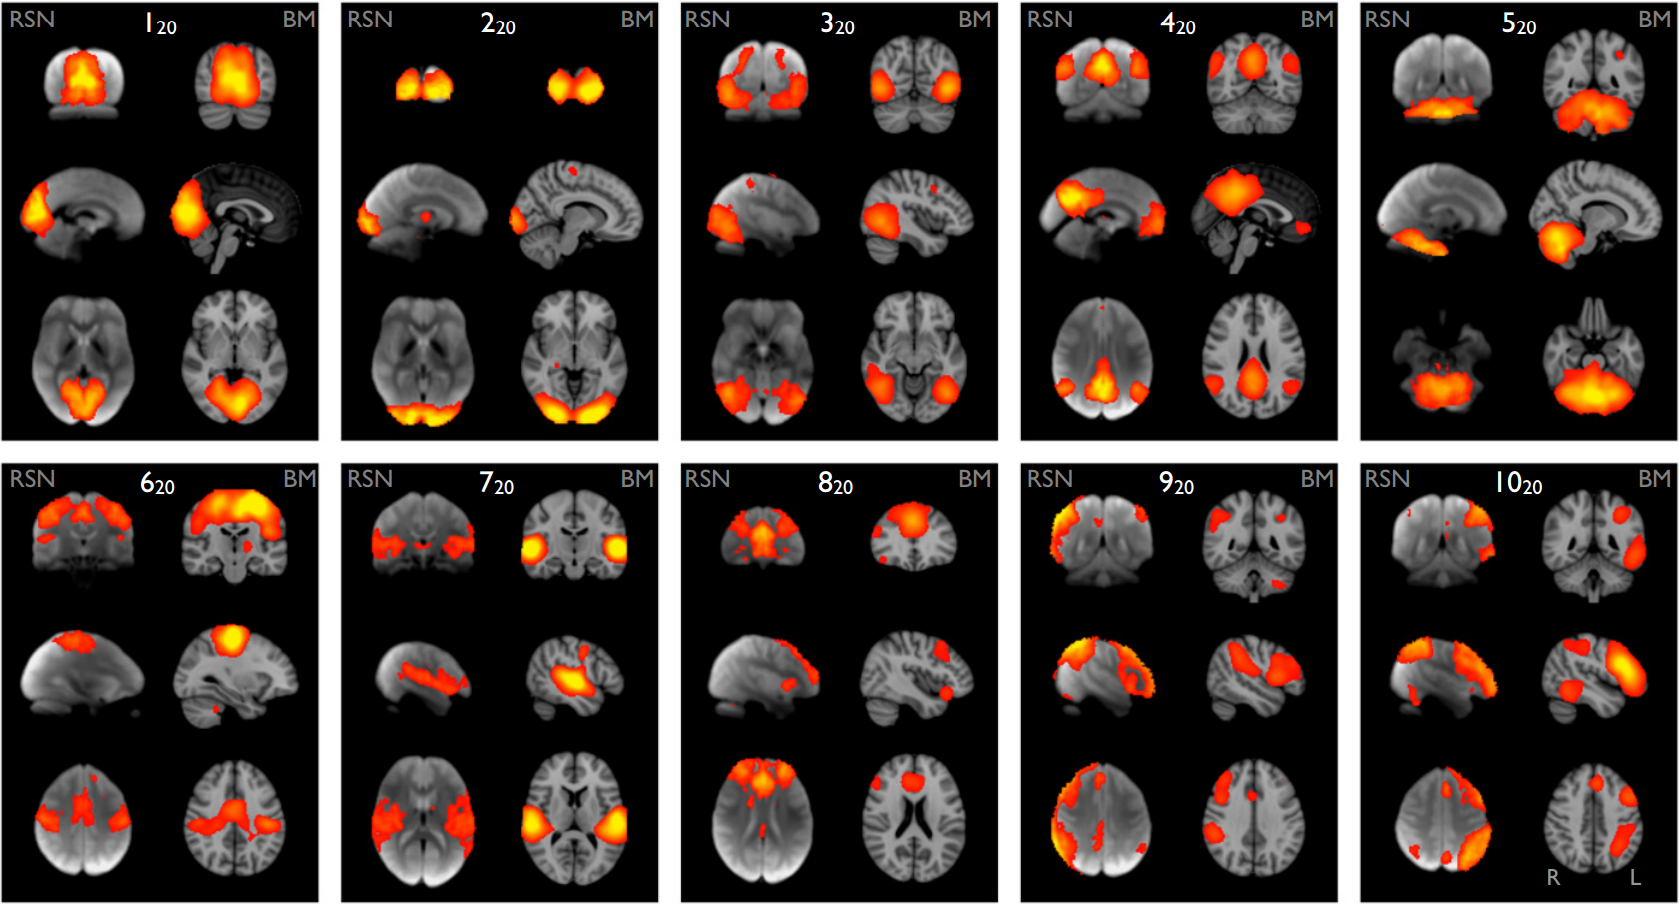
\includegraphics[width=\linewidth]{./images/intro/smith.png}\caption{10 of 20 functional networks derived from two different fMRI resting state datasets. Networks are as follows: 1-3)  medial, occipital and lateral visual networks. 4) Default mode network 5) Cerebellum 6) Sensorimotor 7) Auditory 8) Executive control 9-10) Left and Right frontoparietal networks. Networks labelled RSN were derived from a internal fMRI study and those labelled BM were from the BrainMap \citep{Laird2005} dataset, highlighting the robust nature of resting state functional networks.  Figure reproduced from \cite{Smith2009}.}\label{fig_intro_1}
	\end{center}
\end{figure}

\section{Electrophysiological networks}
There is no question about the importance of fMRI's contribution to functional connectivity, but there are limitations when using it to investigate brain function. The first is that the BOLD response is a haemodynamic process and is therefore an indirect reflection of electrical brain activity. Artefactual correlation between spatially separate regions could result purely from changes in haemodynamics; for example, fluctuations in heart rate or respiration are known to evoke BOLD changes that are correlated across cortical regions and resemble, to a degree, functional networks \citep{Birn2012,Murphy2013,Tong2015}. This effect become more pronounced when investigating non-stationary functional connections, as it has been shown that it can track blood flow along vascular pathways from a region of interest \citep{Webb2013}. Secondly, the latent nature of the oxygenated blood delivery ($\sim$ 5-8 s after a neural event) means that many of the dynamical processes are obfuscated. To return to the catching of a ball analogy, we would only see the activity several seconds after the ball has been caught! These technical limitations can be circumvented if we look to assess functional connectivity using electrophysiological measurements. One such measure, magnetoencephalography (MEG; \citealp{Cohen1968}), non-invasively measures the extracranial magnetic field associated with synchronised neural current flow. Application of appropriate mathematical modelling to these field data allows 3D imaging of electrical activity in the human brain. In short MEG uses an array of superconducting quantum interference devices (SQUIDS; \citealp{Zimmerman1970}) placed around the head to measure the tiny changes in the magnetic fields ($\sim10^{-14}$ T) from neurons. Whilst the technology is decades old, it has really only come of age since the beginning of the 21\textsuperscript{st} Century. This is part fuelled by improved hardware; systems now allow whole head coverage utilising $\sim$ 300 sensors, allowing for advances in mathematical algorithms to, for example, better localise MEG data within the brain, than would be possible with only partial coverage of the head. Secondly, a crucial factor has been an increase in affordable computer processing power to handle the vast amount of data produced by an MEG experiment. MEG possesses good spatial resolution (typically $\sim5$ mm, but given good experimental practices this can be pushed as high as 2 mm \citep{Troebinger2014}), this betters what even high density EEG systems can achieve, which are limited by the conductive properties of the skull smearing the electric fields which pass through it. This, combined with the excellent temporal resolution of MEG, makes it attractive to researchers who want make a non-invasive assessment of brain electrophysiology. Even prior to the growth in functional connectivity analysis, there was a large body of work probing relationships between the haemodynamic response and changes in amplitude of neural oscillations. The primary finding is that good spatial correlation exists between haemodynamic and electrical oscillatory activity, across a broad range of frequencies \citep{Logothetis2001,Singh2002,Moradi2003,Brookes2005,Mukamel2005,Winterer2007,Muthukumaraswamy2008,Zumer2010,Stevenson2011,Stevenson2012}. The first fully independent electrophysiological demonstration of functional networks in the human brain was presented by \cite{Laufs2003}, where known fMRI attentional networks were correlated with EEG sensor timecourses in a concurrent fMRI/EEG study. In 2007 a study by \cite{Mantini2007} this process was taken further by deriving networks in fMRI using Independent Component Analysis and then charactering showing that each network possessed unique electrophysiological spectral signatures observed from concurrent EEG recordings. 

More recently, several studies have been able to replicate the topographies of fMRI functional connections using MEG at the source level. In 2010, de Pasquale and colleagues used MEG to find the dorsal attention network and the default mode network using seed based connectivity \citep{dePasquale2010}. In 2011, a multimodal study in fMRI and MEG showed that the motor network could be imaged in both modalities following a finger tapping exercise \citep{Brookes2011a}. The same year, the same group followed this by performing a temporal independent component analysis (tICA) on MEG resting state data. They found they could match 8 of the resultant functional networks in MEG with fMRI derived networks \citep{Brookes2011}. Finally, using a combination of seed-based and graph theoretical measures \cite{Hipp2012}, showed that MEG functional networks showed clear spatial and spectral structure. Studies like this have begun to confirm that the networks observed in fMRI have an electrophysiological basis.

\section{Towards the dynamic connectome}\label{sec_1_dyn}

In almost all functional connectivity studies, the methods are used to probe the interdependency between regions to assess temporal correlation over the duration of an entire experiment. The result of this is a statistic generated from minutes or even hours of data; this approach assumes that functional connectivity is stationary in time. However, analyses of functional timeseries (by say, assessing signal variance over time) show that they are themselves non-stationary, and therefore implies that a non-stationary analysis of functional connectivity is necessary. A growing body of studies have stated to confirm that this is indeed the case. fMRI has been used to investigate non-stationarity in functional connectivity. In a study by \cite{Chang2010} the authors employed a sliding window analysis, in which connectivity was assessed in many small time windows, that were allowed to shift in time across an fMRI dataset. Their results revealed that the strength of functional connectivity varied markedly, depending on which time window they assessed. Using fast acquisition methods in fMRI, \cite{Smith2012} showed that previously established networks were in fact formed from multiple transient components. \cite{Allen2014}, also using a sliding window analysis, and showed significant departures from the spatial structure of canonical RSNs, if transient connectivity was taken into account. These promising results (and many others, see \citealp{Hutchinson2013} for an extensive review) are in agreement with the hypothesis of a dynamic connectome, and suggest that future neuroimaging methodologies should be developed to capture transient rather than time averaged connectivity. However, as mentioned earlier, the sluggish nature of the haemodynamic response masks much of the temporal nature of connectivity. The millisecond temporal resolution of MEG therefore offers immediate advantages.

A small but growing number of studies are now beginning to show that the dynamic assessment of electrophysiological connectivity using MEG confirms the existence of significant non-stationarity. In early work, a study by \cite{dePasquale2010} showed that by incorporating non-stationarity into their data processing pipeline, they were able to better resolve the default mode and dorsal attention networks. Brookes and colleagues showed that, in the sensorimotor network, a sliding window analysis demonstrated significant fluctuation in the strength of functional connectivity between motor cortices \citep{Brookes2011a}. This work
was extended by \cite{Baker2012} who used a similar technique to reveal a bi-stable nature of envelope correlation, with near-zero levels of connectivity interspersed with periods of high connectivity. A further study by \citep{Baker2014} was able to exploit the excellent temporal resolution of MEG more fully, using a Hidden Markov Model (HMM). This approach, which identifies the points in time at which unique patterns of electrophysiological activity recur, revealed transient (100–200 ms) brain states with spatial topographies similar to RSNs. Studies like these allow for the probing of functional connectivity at temporal scales previously unachievable. 

\begin{figure}
	\begin{center}
		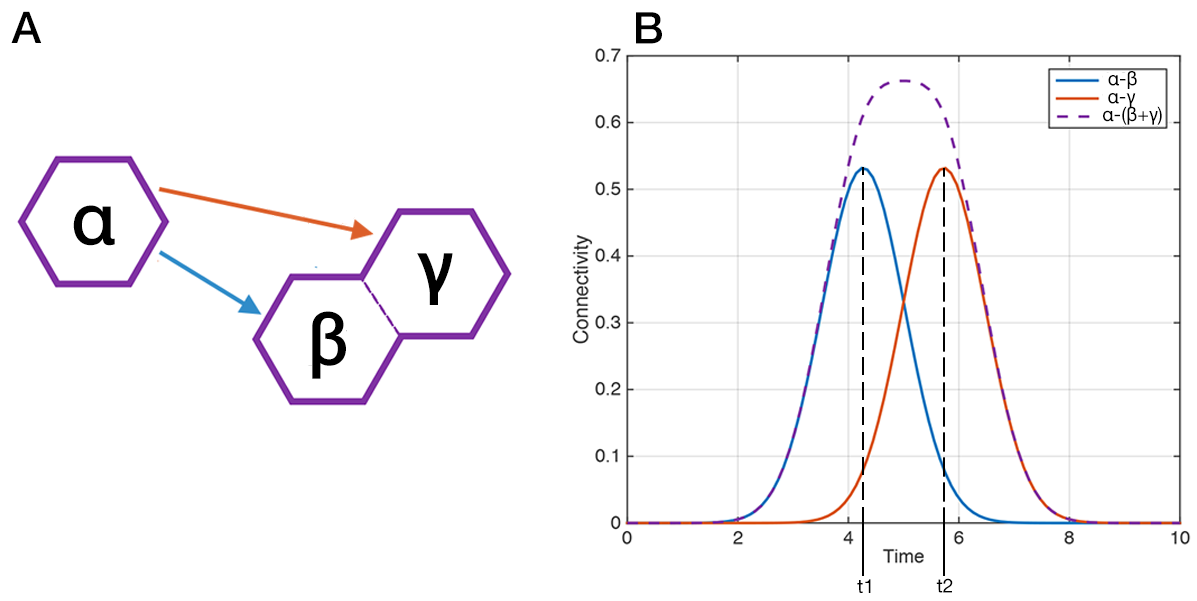
\includegraphics[width=\linewidth]{./images/chapter3/fig_conn_2.png}
		\caption{A cartoon network to highlight the confounds of insufficient voxel selection on functional connectivity results. A) The morphology of a two-cluster network with three nodes. The orange and blue arrows represent the two connections assessed. B) The results from both tests reveal the two individual connections which form and dissolve during their assessment.}\label{fig_3_b}
	\end{center}
\end{figure}

However, the existence of temporal structure in functional connectivity brings with it considerations for the spatial dynamics of RSNs. Consider Figure \ref{fig_3_b}A which shows a simple model of a network: at time point 1, regions α and β exhibit a strong connection; at time point 2, regions α and γ exhibit a strong connection. This simple example reflects a transient spatial reorganisation of the network, and illustrates how temporal and spatial analyses can be confounded. Firstly, if connectivity is computed over all time, for example via seed based correlation taking region α as the seed, then this will result in the blurring together of regions β and γ. Secondly, if a sliding window analysis is undertaken between point locations (e.g. between regions α and β) then this captures a dynamic change in functional connectivity (i.e. it results in the blue line in Figure \ref{fig_3_b}B), but misses the fact that the spatiotemporal dynamics actually reflect a spatial reorganisation. Thirdly, if cluster metrics are undertaken such that regions β and γ are collapsed together, then this results in temporal blurring of the dynamics (i.e. the result is the purple dashed line in Figure \ref{fig_3_b}B). Even if a system to capture all this non-stationary connectivity is devised, it has been shown that poor experimental design and not carefully controlling for false positives can mean that measurement errors (in both acquisition and analysis) can be misrepresented as dynamic changes in connectivity. It therefore follows that methods to capture and assess the true nature of spatiotemporal network dynamics are non-trivial.

\section{Thesis overview}
The aim of this thesis is to exploit the unparalleled spatiotemporal resolution of electrophysiology (with particular emphasis on MEG) to characterise the dynamic properties of functional connectivity. It is hoped that the novel methods introduced within this text, demonstrated on healthy volunteers, could ultimately be used to assess differences in functional connectivity in clinical populations in the future. To confidently assess functional connections, even in the stationary domain with MEG, is not a trivial task and beset with many technical hurdles. This thesis can be split into two sections, the first describes the methods to overcome many of the confounds from data acquisition to connections estimation.

\begin{itemize}
	\item \textbf{Chapter 2} reviews the physics behind signal acquisition in MEG. It covers what we believe is the best explanation for the neural origin of the MEG signal, followed by a discussion of the physics behind SQUIDs, which allow us to detect femtoTelsa sized changes in the magnetic field strength. Next the methods which allow us to remove sources of electromagnetic interference several orders of magnitude larger than the biomagnetic data are discussed. Finally the protocols used to acquire the MEG data in this thesis are laid out.
	\item \textbf{Chapter 3} explains the need for projecting MEG data back into source space, to produce volumetric images of neural current in the brain. We then review the electromagnetic models used to perform source reconstruction by solving the MEG forward and inverse problems. The chapter concludes with a short experimental investigation into whether the choice of source reconstruction methods has a profound effect on functional network mapping. 
	\item \textbf{Chapter 4} reviews the literature on the popular methods used to assess functional connectivity in MEG and some of their applications. It then introduces the technical confound of signal leakage, a consequence of insufficient forward and inverse problems, which introduces artefactual functional connections in MEG. The nature of this leakage is characterised though a series of analytical models and simulations, before reviewing methods to ameliorate the effect it has on experimental studies. 
\end{itemize} Having discussed methods to overcome the many technical challenges assessing functional connectivity with MEG presents, we then introduce the novel methods to capture the non-stationary nature of the connectome.

\begin{itemize}
	\item \textbf{Chapter 5} introduces a pipeline to assess dynamic connections in 5 dimensions: space, time and frequency. Using canonical correlation analysis we demonstrate that we can assess functional connections between two large brain volumes and reveal the dynamic nature of network subconnections in a single subject.
	\item \textbf{Chapter 6} uses the same pipeline to investigate the workings of the sensorimotor network across two different MEG studies. We reveal that the functional networks previously discovered are in fact the temporal aggregate of functionally specific subnetworks, which rapidly form and dissolve based on present mental state.
	\item \textbf{Chapter 7} introduces a different method to assess dynamic functional connections with whole brain coverage. Based on the method of cortical parcellation, we reduce the problem of trying to assess all-to-all functional connectivity, and then use it to track the dynamical behaviour of functional networks across motor and working memory studies.
\end{itemize} Finally, in \textbf{Chapter 8}, concluding remarks are presented, along a brief outline of potential future work.
	
